% !TEX encoding = UTF-8 Unicode
\documentclass[a4paper,twoside,twocolumn,10pt]{article}
\usepackage{abstract} % Style for abstracts in Dept. CSIS, OPU
%\usepackage{abstract4past} % Style for abstracts for the past curriculum

%%%%%%%%%% Designate packages you need %%%%%%%%%%
\usepackage{graphicx} % Enhanced support for graphics
\usepackage{url} % Verbatim with URL-sensitive line breaks
% added
\usepackage{multirow}
%%%%%%%%%% Parameters that should be customized %%%%%%%%%%
% Language (1 = Japanese, 2 = English)
\setlang{1}  % Japanese
% Bachelor or Master (1 = Bachelor, 2 = Master)
\setborm{1}  % Bachelor
% Fiscal year
\setfy{2021}
% Group number
\setgnum{1}
% Presentation order
\setorder{5}  % ヒエンさんはここ8かな
% Increase page number (optional)
%% \pplus{1}

% Title
\title{皮肉データセットを用いた深層学習による皮肉推定手法}
% Author
\author{多田 瑞葵}
%%%%%%%%%% Parameters that should be customized (end) %%%%%%%%%%

\begin{document}
\maketitle  % Insert title
\small

% memo
% 章は「はじめに」「SARC データセット」「実験」「結果と考察」になるかな?
% 実験の章にモデルか処理の図を入れれば良いかな

%%%%%%%%%%%%%%%%%%%%%%%%%%%%%%
\section{はじめに}
皮肉表現とは,文章の文字通りの意味と書き手の意図とが異なる修辞表現である.皮肉表現の理解は,人間にとっては凡そ容易である一方で,機械にとっては未だ困難である.そのため機械による皮肉推定は,文章の理解や感情分析等の分野でも課題となっている.\par
本研究では皮肉表現にドメイン依存性が存在するという仮説のもと,SARC データセット \cite{khodak-etal-2018-large} を用いて文章の話題ごとの皮肉推定に取り組んだ.また文脈を考慮できるモデルとして深層言語処理モデル BERT \cite{DBLP} を使用した.


%%%%%%%%%%%%%%%%%%%%%%%%%%%%%%
%\section{要素技術}
\section{BERT}
Bidirectional Encoder Representations from Transformers (BERT) は,Transformer による双方向のエンコーダーを用いた言語モデルである.文章を文頭と文末の双方向から学習することによって文脈を理解することを可能としている.様々な事前学習済みモデルが発表されており,ファインチューニングすることで各タスクに応用可能である.本研究では,Wikipedia の英語記事で事前学習されたモデルである bert-base-uncased\footnote{\url{https://huggingface.co/bert-base-uncased}} を使用した.\par
BERT は文の入力に対して,入力された文および文に含まれる各単語に対応する分散表現を出力する.また特殊トークンが用意されており,文頭の“[CLS]”トークンに対応する分散表現を入力された文全体の分散表現とみなして分類問題に使用することができる.\par



%%%%%%%%%%%%%%%%%%%%%%%%%%%%%%
\section{SARC データセット}
本研究では,自己注釈付き Reddit コーパス(Self-Annotated Reddit Corpus; SARC)を使用した.
このデータセットは Reddit\footnote{\url{https://www.redditinc.com}} に投稿されたコメントから構築されており,皮肉ラベルが付与されている.
各コメントには,投稿者の識別子,subreddit と呼ばれる投稿トピック,ユーザ評価,投稿日時,親投稿の情報も付与されている.
親投稿とは,最初の投稿から各コメントに至るまでの一連の投稿であり,全てのコメントは 1 つ以上の親投稿を保持している.
図 \ref{fig:1_data_example} にデータの例を示す.
本研究では,皮肉推定の対象となるコメントと,その直接の投稿元である 1 つの親投稿のコメントを実験に使用した.\par
本研究では SARC 2.0 main の均衡データセットから subreddit ごとのデータセットを作成し,テストデータが 1,500 件以上であった 4 つの subreddit(politics, AskReddit, worldnews, pcmasterrace)を対象に皮肉推定をした.また main からデータをランダムサンプリングした random データセットを作成し,比較対象とした. \par



%%%%%%%%%%%%%%%%%%%%%%%%%%%%%%
\section{実験}
データセットの各コメントが皮肉か非皮肉かの二値分類をした.
まず,コメントを BERT に入力し,出力された分散表現から“[CLS]”トークンに対応する分散表現を取得した.
そして取得した分散表現を線形層に入力し,皮肉か非皮肉かを推定した.
その際,訓練データを用いて BERT をファインチューニングし,テストデータに対する精度を確認した.

%%% figure データサンプル
\begin{figure}[tb]
  \centering
  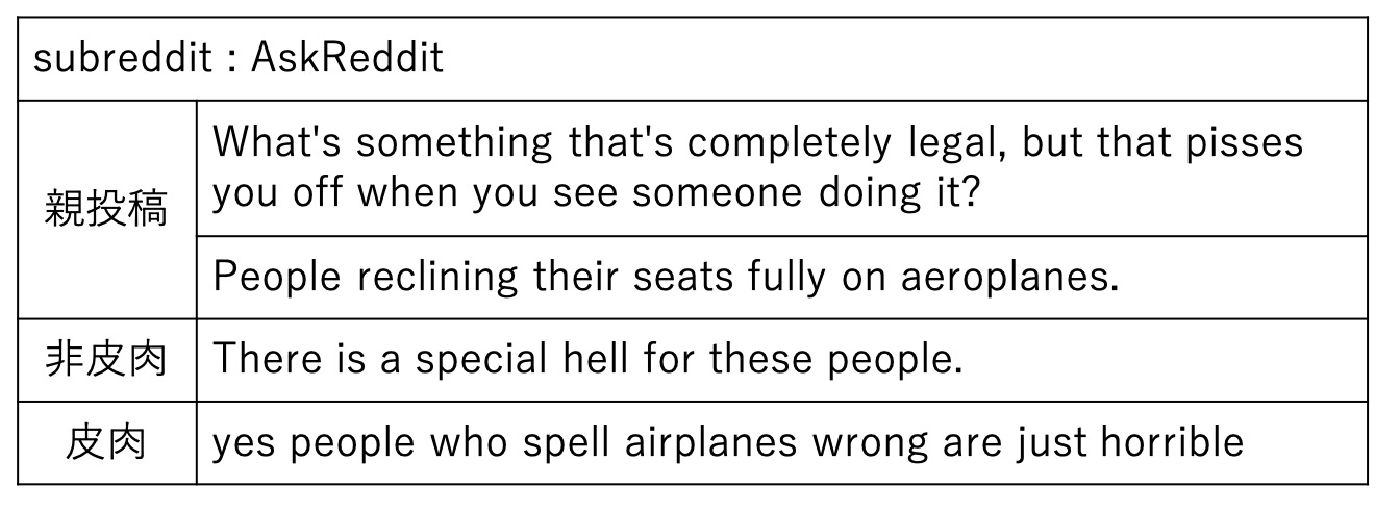
\includegraphics[width=.8\hsize]{data_sample.eps}
  \caption{データセットのデータ例}
  \label{fig:1_data_example}
\end{figure}
% end figure
% 画像の拡張子は .eps にしないといけない
 
%%%%%%%%%%%%%%%%%%%%%%%%%%%%%%
\section{結果と考察}
表 \ref{tb:1_result} にテストデータの実験結果を示す.
太字の項目は random の評価値を上回ったことを示している.politics, worldnews, pcmasterrace の F1 値は random を上回り,politics ではどの評価値においても random を上回る結果となった.
このことから,ドメインごとに皮肉を学習,推定することで,皮肉推定の精度が向上する場合があると考えられる.
一方で,AskReddit ではどの評価値においても random を下回る結果となった.
このことから,AskReddit における皮肉推定が困難であり,データセット全体の推定の際に精度を下げる要因の一つとなることが考えられる.



% 表 \ref{tb:1_result} にテストデータの実験結果を示す.図 \ref{fig:1_matrix} に学習したモデルとデータセットを入れ替えた実験結果を示す.図は縦軸が学習モデル,横軸がデータセットを表している.

%%% table
\begin{table}[tb]
  \caption{実験結果}
  \label{tb:1_result}
  \centering
  \begin{tabular}{c c c c c} \hline

subreddit & Accuracy & Precision & Recall & F1 score\\ \hline
politics & \textbf{0.730} & \textbf{0.722} & \textbf{0.748} & \textbf{0.735} \\
AskReddit & 0.619 & 0.630 & 0.580 & 0.604 \\
worldnews & \textbf{0.690} & 0.655 & \textbf{0.803} & \textbf{0.721} \\
pcmasterrace & 0.648 & 0.635 & \textbf{0.698} & \textbf{0.665} \\ \hline
random & 0.653 & 0.664 & 0.618 & 0.640 \\ \hline

  \end{tabular}
\end{table}
% end




%%%%%%%%%%%%%%%%%%%%%%%%%%%%%%
\section{まとめと今後の課題}
本研究では,BERT を用いた皮肉推定に取り組み,皮肉表現のドメイン依存性について確認した.
皮肉表現にドメイン依存性が存在するという仮説のもと,subreddit ごとのデータセットを作成して皮肉推定をし,精度を比較した.
結果として,subreddit ごとに皮肉推定することで精度が向上したものと低下したものがあり,ドメインを考慮して皮肉推定する手法の有効性と,皮肉推定の困難なドメインの存在を示すこととなった.\par
今後の課題として,ドメインごとの弱学習器を用いたアンサンブル学習によって皮肉推定に取り組むことや,皮肉推定に使用する文脈情報やメタデータを拡大することが挙げられる.




%%%%%%%%%%%%%%%%%%%%%%%%%%%%%%

\bibliographystyle{jabbrvunsrt}
\bibliography{index_ja}
\end{document}





%\clearpage
%\section{作成要領}
%\subsection{卒業研究論文}
%\begin{enumerate}
%\item ページ制限,用紙\\
%  卒業論文概要は A4 版 原則 1 ページとし片面を用いる(2人で両面).
%  特別な場合2ページまで可.
%\item フォーマット\\
%  指定されたLaTeXまたはWordのテンプレートを使用する.
%\item グループ番号とページ番号\\
%  ページの右上に「グループ番号−グループ内通しページ番号」を記入する.
%\end{enumerate}
%
%
%\subsection{設定}
%abstract.texの上部には以下の設定項目があり,各自しかるべき値に変更する.
%%
%\begin{verbatim}
%% Language (1 = Japanese, 2 = English)
%\setlang{1}
%% Bachelor or Master (1 = Bachelor, 2 = Master)
%\setborm{2}
%% Fiscal year
%\setfy{2015}
%% Group number
%\setgnum{3}
%% Presentation order
%\setorder{2}
%% Increase page number (optional)
%%% \pplus{1}
%\end{verbatim}
%%
%Presentation orderは発表順である.
%これが指定されると,卒業研究論文の場合は1人当たり1ページ,
%修士学位論文の場合は1人当たり2ページとしてページ番号が自動的に計算される.
%何らかの事情によりページ番号がずれる場合は,
%$\backslash$pplus\{1\}
%のように指定してページ番号を増加(または減少)させることができる.
%
%\subsection{図表}
%表 \ref{tbl:kuku}は表の例,
%図 \ref{fig:CSIS_logo}は図の例である.
%
%\begin{table}[tb]
%  \caption{表の例:九九}
%  \label{tbl:kuku}
%  \centering
%  \begin{tabular}{|c||c|c|c|c|c|c|c|c|c|} \hline
%    - &  1 &  2 &  3 &  4 &  5 &  6 &  7 &  8 &  9 \\ \hline \hline
%    1 &  1 &  2 &  3 &  4 &  5 &  6 &  7 &  8 &  9 \\ \hline
%    2 &  2 &  4 &  6 &  8 & 10 & 12 & 14 & 16 & 18 \\ \hline
%    3 &  3 &  6 &  9 & 12 & 15 & 18 & 21 & 24 & 27 \\ \hline
%    4 &  4 &  8 & 12 & 16 & 20 & 24 & 28 & 32 & 36 \\ \hline
%    5 &  5 & 10 & 15 & 20 & 25 & 30 & 35 & 40 & 45 \\ \hline
%    6 &  6 & 12 & 18 & 24 & 30 & 36 & 42 & 48 & 54 \\ \hline
%    7 &  7 & 14 & 21 & 28 & 35 & 42 & 49 & 56 & 63 \\ \hline
%    8 &  8 & 16 & 24 & 32 & 40 & 48 & 56 & 64 & 72 \\ \hline
%    9 &  9 & 18 & 27 & 36 & 45 & 54 & 63 & 72 & 81 \\ \hline
%  \end{tabular}
%\end{table}
%
%\begin{figure}[tb]
%  \centering
%  \includegraphics[width=.3\hsize]{CSIS.eps}
%  \caption{図の例:ロゴ}
%  \label{fig:CSIS_logo}
%\end{figure}
%
%\subsection{参考文献}
%pBibTeXの使用を推奨する.
%その場合,同梱されているjabbrvunsrt.bstを使うこと.
%これは,jabbrv.bstのソート機能をオフにしたものである.
%%\cite{SakaiMe, Food, Neko}は使用例である.
%
%\subsection{スタイル}
%Normal, Title, Author, Section, SubSection, SubSubSection, References,
%Table, Verbatim, Enumerate, Itemizeのスタイルが定義されているので、
%適宜使用する。
